\documentclass[12pt,xcolor=svgnames]{beamer}
\usepackage{dsfont,natbib,setspace,changepage,multirow}
\mode<presentation>

% replaces beamer foot with simple page number
\setbeamertemplate{navigation symbols}{}
\setbeamertemplate{footline}{
  \raisebox{10pt}{\makebox[\paperwidth]{\hfill\makebox[20pt]{\color{gray}\scriptsize\insertpagenumber}}}}

% colors
\newcommand{\bk}{\color{black}}
\newcommand{\rd}{\color{red}}
\newcommand{\fg}{\color{ForestGreen}}
\newcommand{\bl}{\color{blue}}
\newcommand{\gr}{\color{gray}}
\newcommand{\sg}{\color{DarkSlateGray}}
\newcommand{\nv}{\color{Navy}}
\newcommand{\theme}{\color{Maroon}}
\setbeamercolor{itemize item}{fg=gray}

% common math markups
\newcommand{\bs}[1]{\boldsymbol{#1}}
\newcommand{\mc}[1]{\mathcal{#1}}
\newcommand{\mr}[1]{\mathrm{#1}}
\newcommand{\bm}[1]{\mathbf{#1}}
\newcommand{\ds}[1]{\mathds{#1}}
\newcommand{\indep}{\perp\!\!\!\perp}

% spacing and style shorthand
\newcommand{\sk}{\vspace{.5cm}}
\newcommand{\R}[1]{{\tt \bl #1}}
\newcommand{\til}{{\footnotesize$\bs{\stackrel{\sim}{}}$ }}
\setstretch{1.1}

\begin{document}

\setcounter{page}{0}
{ \usebackgroundtemplate{\includegraphics[height=\paperheight]{/Users/mtaddy/Dropbox/inputs/phoenix}}
\begin{frame}[plain]
\begin{center}


{\bf \huge \theme The Gamma Lasso }

\vskip 1cm
Matt Taddy, University of Chicago Booth School of Business

\vskip .2cm
\texttt{faculty.chicagobooth.edu/matt.taddy/research}

\end{center}
\end{frame} }

\begin{frame}

{\bf \theme Big data analysis examples}

\vskip .25cm
Consider massive $n\times D$ count matrices $\bm{C}$, \\paired with an $n\times K$ attribute matrix $\bm{V}$. 


\vskip .25cm
{\nv Congressional Speech }
\vskip .1cm
{\footnotesize
\begin{tabular}{|c|c|c|c|c|c|c}
Name & Congress & State & Party &  Death Tax & Estate Tax & $\cdots$
\\ \hline
T. Cruz & 113 & TX & {\sf gop}  & 18 &
  0 &  \\ 
C. Schumer & 113 & NY & {\sf dem}  & 1 &
  8 & 
\end{tabular}}

\hskip 5cm $\ddots$


{\nv Web Browsers }
\vskip .1cm
{\footnotesize
\begin{tabular}{|c|c|c|c|c|c}
ip address & purchases &  nytimes.com & wsj.com & msnbc.com
& $\cdots$ \\ \hline
212.135.123.24 & $\cdots$  &   54 & 0 & 119 & $\cdots$
\end{tabular}}

\hskip 5cm $\ddots$

\vskip .1cm
The dataset is both wide (big $p = D+K$) and long (big $n$).  \\
Its often too large to store in working memory.  

\vskip -.3cm

\end{frame}

\begin{frame}

{\theme \bf Big multinomials}

\vskip .5cm
I analyze such data with high 
dimensional logistic regressions
\begin{eqnarray*}
\bm{c}_i \sim \mr{MN}(\bm{q}_i, m_i)~~\text{with}~~
q_{ij} = e^\eta_{ij}/\sum_l e^{\eta_{il}},~~
\eta_{ij} = \alpha_j + \bm{v}_i'\bs{\varphi}_{j}
\end{eqnarray*}
{where $m_i = \sum_j c_{ij}$ and $\bs{\varphi}_{j}$ 
is $j^{th}$ column of $\bs{\Phi}$}

\vskip .5cm
In addition to meta-data attributes, $\bm{v}_i$ can contain all sorts of fixed effects to account for, say, within speaker dependence.

{\sg We also work on estimation when the $\bm{v}_i$ include latent factors.}

\vskip .25cm
I fit these big multinomials via $D$ independent Poisson log-linear regressions for each column of $\bm{C}$: $\bm{c}^j \sim \mr{Po}(m_ie^{\eta_{ij}})$.

\vskip .1cm And this happens in distribution: on many different machines.
\end{frame}


\begin{frame}

{\bf Making it work: \theme the gamma lasso}


\sk
All of this means that I end up doing {\it many} ($10^5{\tt+}$) big-$n$ independent 
regressions for each column of $\bm{C}$, say $\bm{c}^j$, onto $\bm{V}$.

\sk
Given the dimensions involved, I want to be regularizing.

\vskip .1cm
{\nv
And given communication limits, I want sparsest $\bs{\hat\varphi}$ possible.}

\vskip .1cm
{\theme And with too many models to really validate, I want stability.}

\vskip .2cm
Turns out that blue and red work against each other.
\end{frame}

\begin{frame}

{\bf \theme Penalized estimation}

\sk Dropping $j$ from here on out, this means I need to
quickly solve hundreds of thousands of penalized deviance problems
{\large\[
{\tt min}\{-\log[l({\bs{\varphi}})] + \lambda c(\bs{\varphi})\}.\]}

For MN Inverse Regression, likelihood $l$ is either Poisson or a weighted least squares (i.e. Gaussian) approximation.

\end{frame}



\begin{frame}

{\bf Penalized estimation}

\vskip .5cm Find $\bs{\hat\varphi}$ to minimize
$ \theme \text{-logLHD}(\bs{\varphi}) + \lambda \sum_k c(\varphi_k)$.

\vskip .25cm
$\lambda >0$ is a penalty weight, $c$ is a cost function with min at 0.
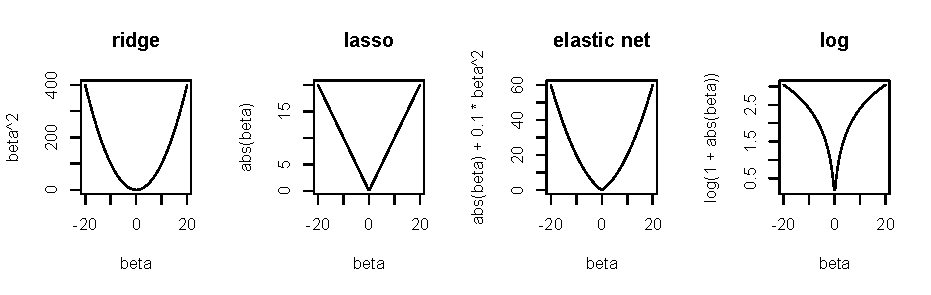
\includegraphics[width=4.25in]{../graphs/penalties}

options: ridge $\varphi^2$, {\theme lasso $|\varphi|$}, elastic net $\alpha\varphi^2 + |\varphi|$,  $\log(1 + |\varphi|)$.

\vskip .25cm
Anything with a spike at zero yields variable selection: 
\\ \hfill $\bs{\hat\varphi}$ will contain exact zeros.~~~~~~~~~~~

\end{frame}

\begin{frame}

{\theme \bf Regularization paths}

\sk
Since we don't know $\lambda$, the penalization doesn't actually {\it do} model selection.  Instead, it {\it indexes} a set of candidate models.

\vskip .1cm
{\gr Think of $\lambda$ as a signal-to-noise filter: like squelch on a radio.}

\sk
Fortunately, path algorithms can do fast fits over grids of $\lambda_t$:
\begin{itemize}
\item Start at $\lambda_1$ large enough that $\bs{\hat\varphi}^1 = \bm{0}$.
\item Incrementally decrease $\lambda_t = \delta \lambda_{t-1}$, $\delta \in (0,1)$.
\item Re-fit coefficients $\bs{\hat\varphi}^t$, using $\bs{\hat\varphi}^{t-1}$ as hot-starts.
\end{itemize}
{\it If} the coefficients change little under small changes to $\lambda$, \\then a full path can take far less time then a single OLS fit.

\vskip .25cm
{\gr The `if' here is stability: continuity of the regularization path.}

\end{frame}

\begin{frame}

{\bf Cost function properties}

\sk
{\nv Ridge} can be optimal for dense signals.
It shrinks the coefficients of correlated variables towards each other.

\vskip .1cm
{\nv Concave} (e.g., log) penalties have diminishing bias, such \\that large signals are estimated with little to no penalty.

\vskip .1cm
{\nv Lasso} is a middle ground.  It tends to choose a single input amongst correlated signals but also
has a non-diminishing bias.  

\sk {\theme Concave penalties are very popular.} \\ Diminishing bias yields oracle theory  and is useful in causal schemes (where you 
want $\varphi$ to suck up all the endogenaity).

\vskip .2cm This comes at the price of stability (i.e., estimation variance),
and computation cost (because of possible multiple minima).

\end{frame}


\begin{frame}

{\bf \theme Concavity and Stability}

\vskip .25cm
Too much penalty concavity causes instability: \\ \hfill small change in $\bm{y}$ (response) lead to large change in $\bs{\hat\varphi}$.

\vskip .25cm  
e.g., Log penalized LS  $\nv (\beta-B)^2 + s\log(1 + \gamma|\beta|)$.

\vskip .25cm  
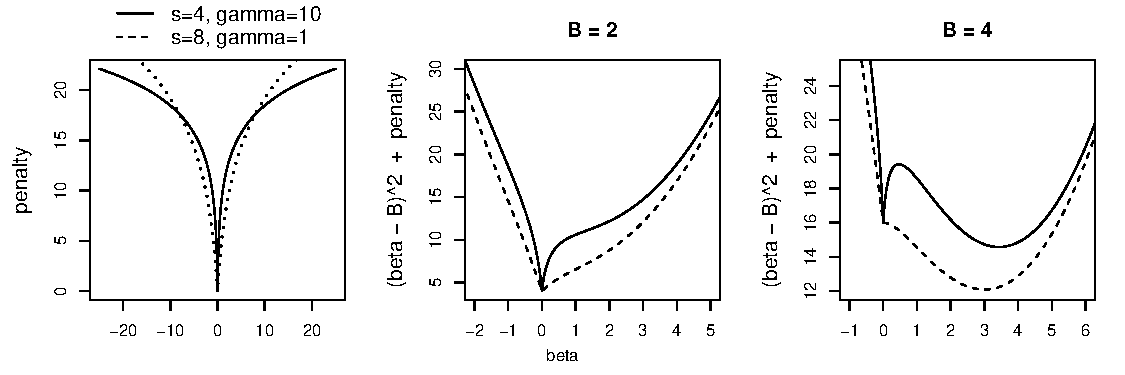
\includegraphics[width=4in]{../graphs/solution}

\vskip .25cm
The solution can jump away from the origin.
\end{frame}

\begin{frame}

{\bf Heuristic concave penalization via \theme the gamma lasso}

\vskip .25cm

Initialize $\bs{\omega}^1 = \bf{1}$ and $\lambda^1 >
0$ with step size
$0 < \delta < 1$.

For $t=1\ldots T:$ 
\vspace{-.25cm}
\begin{align*}
\bs{\hat\varphi}^t &= \mr{argmin}~
l(\bs{\varphi}) + n\sum \lambda^t\omega^t_j|\varphi_j| \\
{\theme \omega^{t+1}_j  }&{\theme = \left(1 + \gamma |\hat\varphi^t_j|\right)^{-1}}, ~~j=1\ldots p,~~ \lambda^{t+1} = \delta \lambda^t
\end{align*}

Each step is just lasso ($L_1$) penalized minimization.  \\But we get diminishing bias since $\omega^{t+1}_j$ decreases with $\gamma |\hat\varphi^t_j|$.

\vskip .1cm
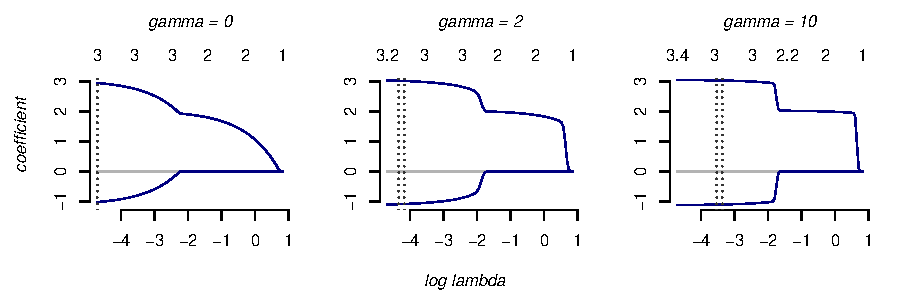
\includegraphics[width=4.1in]{../graphs/gamlr_eg}
\vskip -1cm
\end{frame}


\begin{frame}

This simple little heuristic is my guide to concave penalties.

\vskip .35cm
{\theme Bayes:} under Laplace-gamma prior 
$\mr{La}\left(\varphi ; \tau\right)\mr{Ga}\left(\tau; s,\gamma^{-1}\right)$, the conditional MAP is $\hat\tau | \varphi = \gamma s/(1 + \gamma |\varphi|)$.  

\vskip .2cm Writing $s = n\lambda/\gamma$, GL uses this MAP for $\hat\tau^t_j$ given $\hat \varphi^t_{j-1}$.

\vskip .35cm 
{\theme Log penalty:} true joint MAP of this joint prior implies $s\log(1+\gamma|\varphi|)$ costs; as $\delta \rightarrow 1$ that's what GL approaches.

\vskip .35cm 
{\theme Adaptive lasso:} this is reweighted $L_1$ penalization: it is a specific version of an adaptive lasso.
{\nv I call it `path adaptation'.}


\vskip .35cm 
The GL is a `one-step estimator' in the first two setups, \\and the AL can be cast in this way ({\small Zou{\tt +}Li AoS 08}).  

\vskip .1cm
{\gr For more, see the GL paper on arXiv: it is a review.}


\end{frame}


\begin{frame}

{\bf \theme Concavity and Stability }


\vskip .25cm The $\gamma$ parameter governs how quickly bias disappears:\\
\hfill $\gamma=0$ is the lasso, and $\gamma = \infty$ is subset selection.


\sk
{\nv How stable is the procedure?}

\vskip .25cm
GL has a nice type of theoretical stability for all $\gamma < \infty$:\\ \hfill  Lipschitz continuity with respect to jitter in the response $\bm{y}$.

\vskip .15cm
{\gr [$f$ is Lipschitz continuous if  $ |f(b_1)-f(b_2)| \leq
L|b_1-b_2| $ for some finite constant $L$ on all $b_1,b_2$ in the domain of
$f$.]} 

\vskip .15cm
Intuitively, this requires Lipschitz regularization paths.

\vskip .25cm
{\nv Sub-optimality of the one-step-estimator gives us this stability.}

\end{frame}


\begin{frame}

Be careful: Lipschitz does not guarantee `practical' stability.

\vskip .25cm
e.g., Making $\gamma$ too big causes timings to blow up.
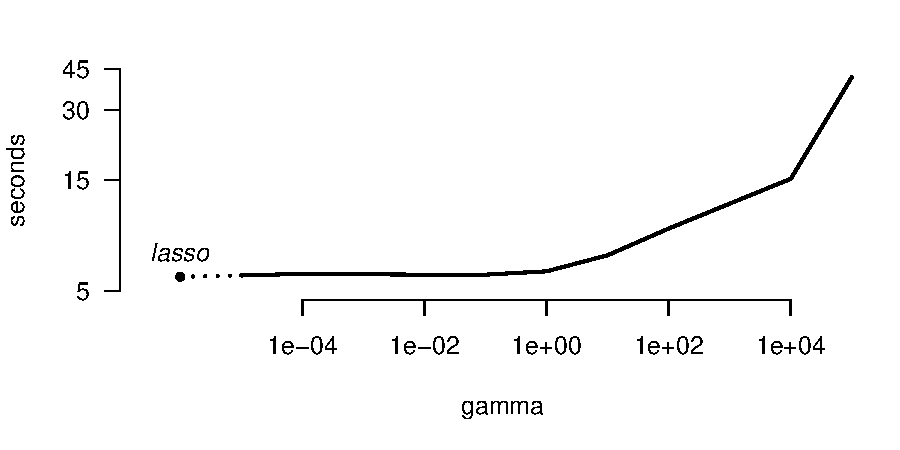
\includegraphics[width=4in]{../graphs/nhl_time}

This is because $\bs{\hat\varphi}^{t-1}$ become bad hot-starts 
for $\bs{\hat\varphi}^t$.

\end{frame}

\begin{frame}

{\bf  $\lambda$ just indexes models.  \theme How do you choose?}

\vskip .2cm
~~~~~~~~~~~e.g., AIC = deviance($\bs{\hat\varphi}$) + 2$df$.

\vskip .5cm
Useful benefit of Lipschitz: use Stein's $df = \ds{E}\left[\sum_i \partial \hat
y_i/\partial y_i\right]$.

\vskip .25cm
Zou et al. 2007 apply this with lasso ($L1$) penalties
\[
\ds{E}\left[ \ds{1}_{[|g_j|<\tau_j]} \right] \approx \sum_j |g_j| < \omega_j\lambda 
\]
\vskip -.35cm
where $g_j$ is $\partial l /\partial x_j |_{\hat \varphi_j=0}$.

\vskip .5cm
Use the Bayesian model to get heuristic version for GL:
\[\nv
\widehat{df} = \sum_j \pi(|g_j| < \omega_j\lambda) \gr = \sum_j \mr{Ga}(|g_{j}|;~ n\lambda/\gamma, 1/\gamma).
\]
\vskip -1cm

\end{frame}

\begin{frame}

{\bf An example: \theme NHL hockey players}

\vskip .25cm
Every goal back to 2002-2003:
64540 goals and 2302 players.

\vskip .25cm
Our `regression plus-minus' model {\gr({\small Gramacy, Jensen, Taddy})}:
\[
\mr{logit}\left[\mr{p}(\text{home~team~scored~goal}~i)\right] = \alpha +
\bm{u}'\bs{\phi} + \bm{x}'\bs{\beta}, 
\]


$x_{ij}=1$ if player $j$ was on the home team and on ice for goal $i$, $x_{ij}=-1$ for away player
$j$ on ice, and $x_{ij}=0$ otherwise.  

\vskip .1cm 
$\bm{u}$ is a vector of indicators for special-teams scenarios.

\vskip .25cm {\nv $\Rightarrow \beta_j$ is the  effect of a player on the log odds
that, given a goal has been scored, the goal was scored by his team.}

\vskip .25cm
We'll fit a GL path  for $\bs{\beta}$, leave $\bs{\phi}$ unpenalized.

\end{frame}

\begin{frame}

{\bf \theme Hockey GL paths}

\vskip .5cm
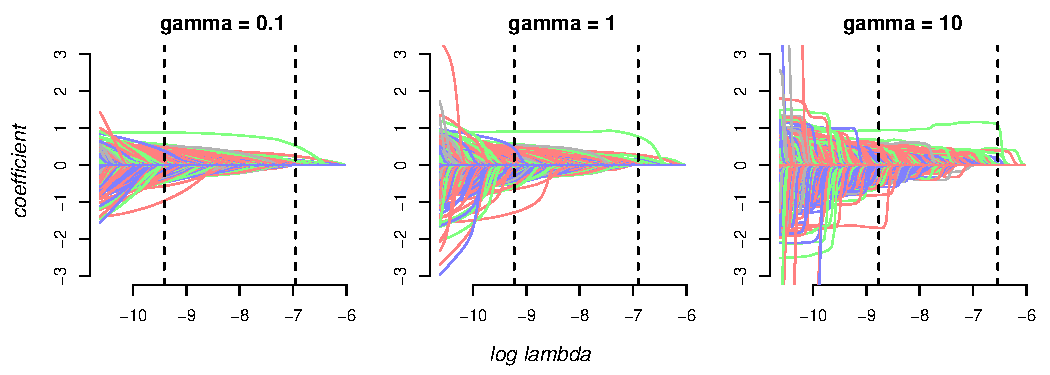
\includegraphics[width=4.25in]{../graphs/nhl_paths}

\sk
Minimum AIC and BIC are marked with the  vertical lines.

\vskip .1cm
grey:goalie, blue:defense, green:center, red:winger.

\end{frame}

\begin{frame}


{\bf \theme Hockey IC surfaces}

\vskip .5cm
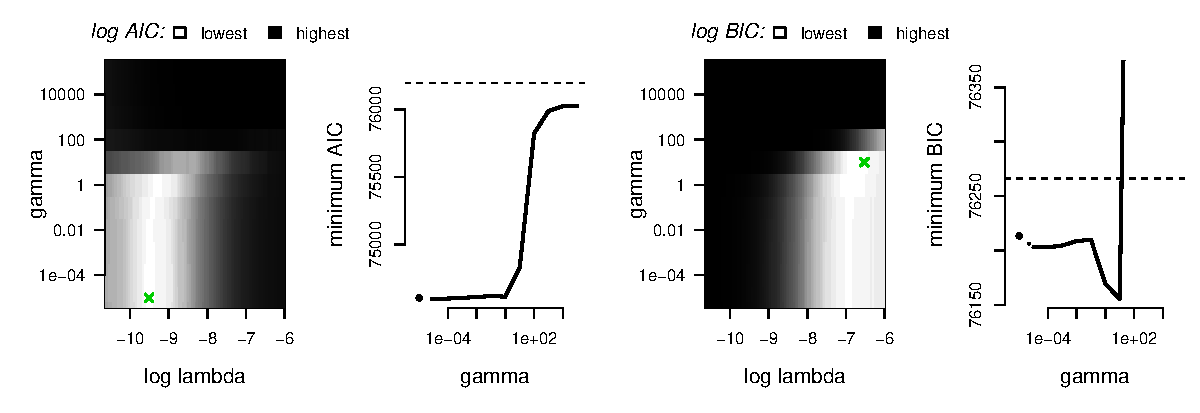
\includegraphics[width=4.25in]{../graphs/nhl_ic}

\vskip .5cm
AIC favors dense high-shrinkage models, \\BIC likes sparse low-shrinkage.

\vskip .25cm
Both seem to hate instability.
\end{frame}

\begin{frame}

{\bf \theme Hockey 20-fold CV}

\sk
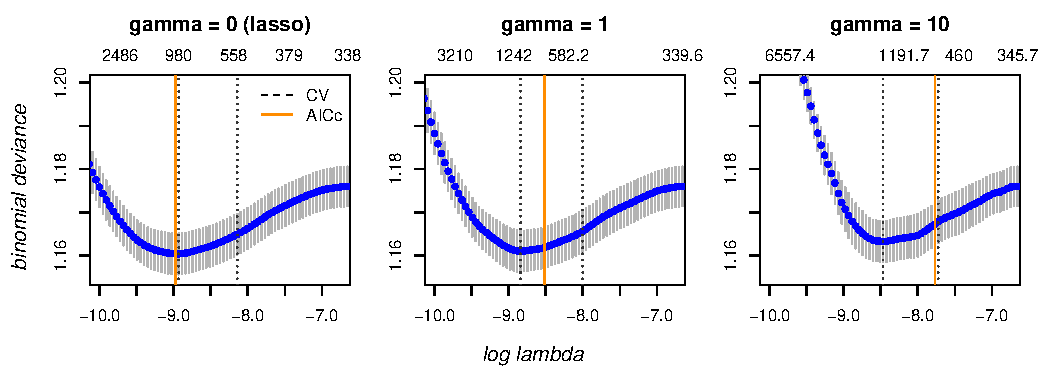
\includegraphics[width=4.25in]{../graphs/nhl_cv}

\sk
Some predictive benefit from small $\gamma>0$, \\and (we find) improved interpretability.  

\vskip .2cm
For larger $\gamma$, you just get more variability.

\end{frame}

\begin{frame}[fragile]

{\bf \theme BIC selected player coefficients}
{\scriptsize
\begin{verbatim}
  PETER_FORSBERG       MARIAN_HOSSA   PAVEL_DATSYUK       HENRIK_SEDIN 
           0.768              0.276           0.268              0.221 
NICKLAS_LIDSTROM        ZDENO_CHARA   SIDNEY_CROSBY  DANIEL_ALFREDSSON 
           0.137              0.134           0.115              0.114 
       DAN_BOYLE      NATHAN_HORTON    JOE_THORNTON     JONATHAN_TOEWS 
           0.114              0.097           0.092              0.085 
   ALEX_OVECHKIN       RYAN_GETZLAF    CHRIS_KUNITZ       JASON_ARNOTT 
           0.075              0.066           0.052              0.039 
    ALEX_TANGUAY VINCENT_LECAVALIER  MARIAN_GABORIK        ZACH_PARISE 
           0.036              0.033           0.019              0.015 
  ROBERTO_LUONGO 
           0.002 
\end{verbatim}}

All total stars for BIC at  $\gamma=10$.  \\
In contrast, AIC at $\gamma=10$ selects 350 good and bad players.

\end{frame}

\begin{frame}

{\bf \theme in conclusion ...}

\vskip .25cm Multinomial Inverse Regression is useful for HD counts.

\vskip .25cm IR in big $D$ requires many penalized regressions.  
\begin{itemize}
\item Concave penalties are great: diminishing bias, extra zeros.
\item But they are not worth the price of instability.
\item The GL is a fast and relatively stable option.
\item Be careful with the theory vs reality disconnect.
\item A penalty just indexes models: {\nv you need to choose, and we only have good tools to do so if the routine is stable.}
\end{itemize}


\sk
\begin{center}
\huge Thanks!
\end{center}
\end{frame}

\end{document}
